\newpage
\section{Tonic, Dominant, Octave}

Someone once told me ``Music is how math sounds.'' I'm not totally
sure I believe them, but maybe there is some truth to what they are
saying. Sound is made by compression waves in the air. Loosely
speaking, the closer the compression waves come, the higher the pitch
the sound is that we hear. We visualize these compression waves with a
picture like this:
\[
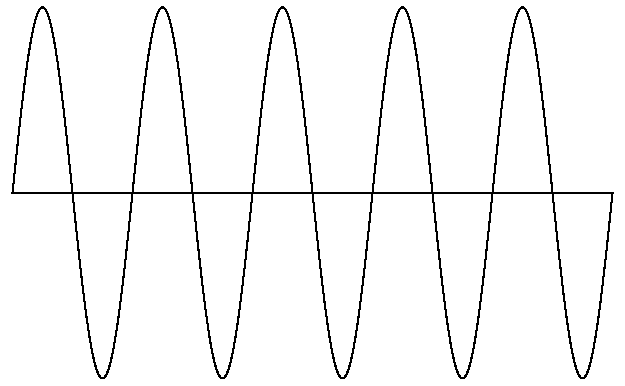
\includegraphics[width=3in]{../graphics/basicWave.pdf}
\]
The peaks of the waves above represent high-pressure points where the
air is very compressed, and the troughs of the waves above represent
low-pressure points, where there are very few air molecules. 

Let's call a sound produced by a single compression wave a \index{tone}
\textit{tone}. When two tones are played at the same time, their waves
act together like the sum of the individual waves. Let's
see this in action. If we play the following two tones at the same
time,
\[
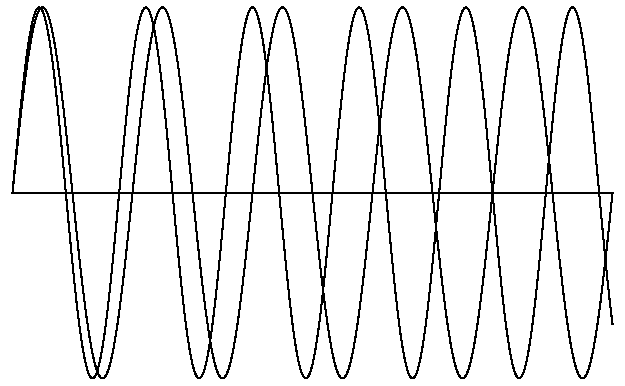
\includegraphics[width=3in]{../graphics/superComb.pdf}
\]
we end up with 
\[
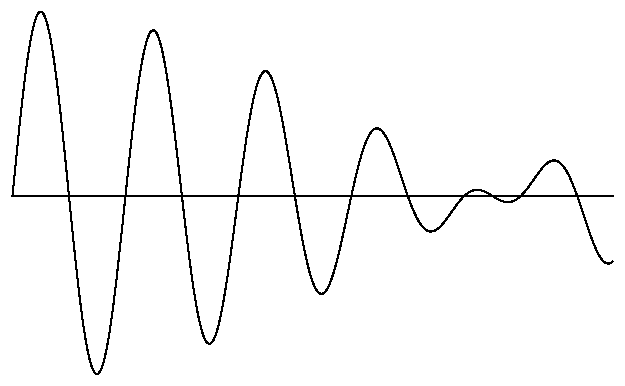
\includegraphics[width=3in]{../graphics/superSum.pdf}
\]
which is nothing more than every point on the first graph added to
every point on the second graph. See how when the waves line up
nicely, we get a nice big wave? See how when the waves disagree, our
wave dwindles down to nothing?

Since the time when people started making sounds, we've noticed that
some tones sound better together than others. There is an easy
rule-of-thumb that will tell you when two tones will sound ``right''
together. If the graph of both waves combined has a lot of beats \index{beats}
then it will probably sound ``wrong,'' see the example below:
\[
\begin{tabular}{ccc}
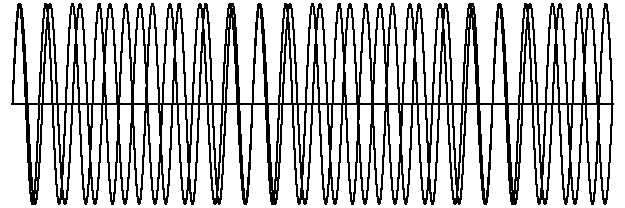
\includegraphics[width=2in]{../graphics/minorComb.pdf}
 & \raisebox{4ex}{\huge$\Rightarrow$} &
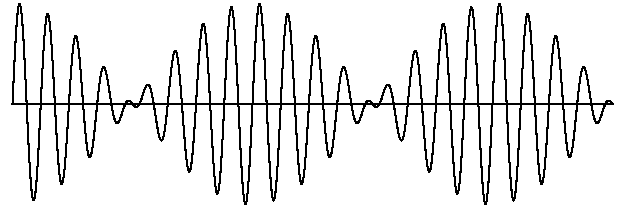
\includegraphics[width=2in]{../graphics/minorSum.pdf}\\
& & beats
\end{tabular}
\]
If the beats are hard to see, then it will sound ``right.'' You can
see this in the following example:
\[
\begin{tabular}{ccc}
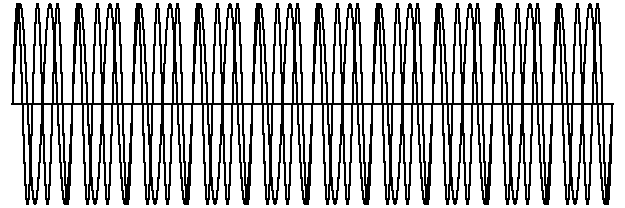
\includegraphics[width=2in]{../graphics/fifthComb.pdf}
 & \raisebox{4ex}{\huge$\Rightarrow$ }&
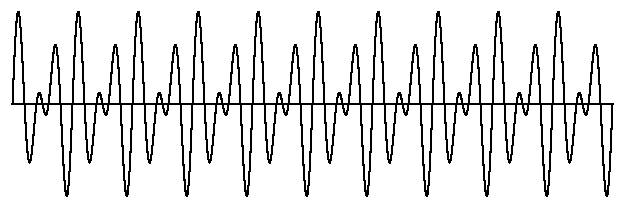
\includegraphics[width=2in]{../graphics/fifthSum.pdf} \\
& & no beats
\end{tabular}
\]
Now let's define some words:

\begin{dfn} 
The \textbf{wavelength}\index{wavelength!sinusoidal wave} of a
sinusoidal wave is length of a complete wave, the distance from peak
to peak or the distance from trough to trough.
\end{dfn}

\begin{dfn} 
The \textbf{frequency}\index{frequency!sinusoidal wave} of a sinusoidal
wave is the number of complete waves per unit time.
\end{dfn}

If we're talking about sound waves, then wavelength and frequency are related by the following equation:
\begin{equation}\label{E:sin}
w_s \cdot f = s\qquad\text{where}\qquad
\begin{tabular}{l}
$w_s$ is the wavelength of the sound wave\\
$f$ is the frequency \\
$s$ is the speed of sound 
\end{tabular}
\end{equation}



\begin{dfn} 
The tone that you start with is called the
\textbf{tonic}.\index{tonic}
\end{dfn}

So let's start with the tonic, and add a tone whose wavelength is half
that of the tonic:
\[
\begin{tabular}{ccc}
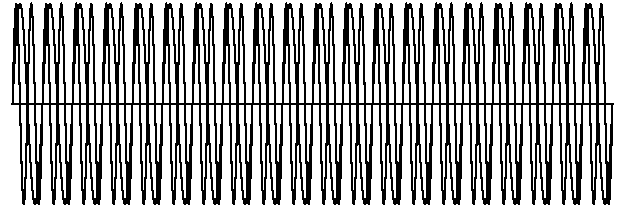
\includegraphics[width=2in]{../graphics/octaveComb.pdf}
 & \raisebox{4ex}{\huge$\Rightarrow$ }&
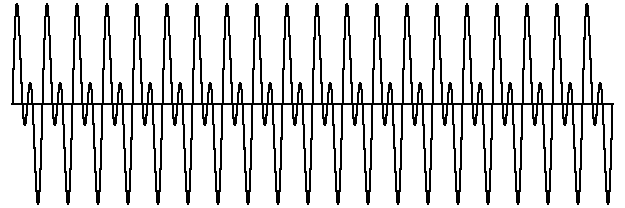
\includegraphics[width=2in]{../graphics/octaveSum.pdf}
\end{tabular}
\]
That looks like it sounds really ``right,'' as there are no beats to be seen.

\begin{dfn}
The tone whose wavelength is half that of the tonic is called the
\textbf{octave}.\index{octave}
\end{dfn}

For some reason, the human ear and brain work together to identify the
tonic and octave as \textit{the same} tone, with the octave just being
twice as high. Now let's get a little crazy, we'll start with the
tonic, and add a tone whose wavelength is $2/3$ that of the tonic:
\[
\begin{tabular}{ccc}
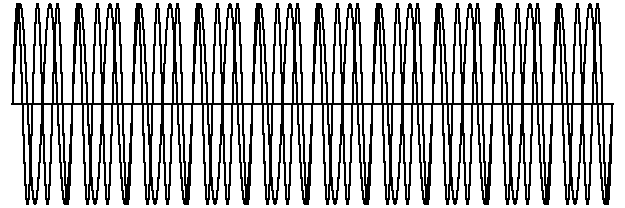
\includegraphics[width=2in]{../graphics/fifthComb.pdf}
 & \raisebox{4ex}{\huge$\Rightarrow$ }&
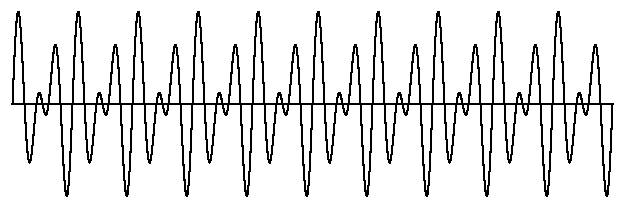
\includegraphics[width=2in]{../graphics/fifthSum.pdf}
\end{tabular}
\]
That looks like it sounds ``right'' too, no beats again.

\begin{dfn}
The tone whose wavelength is $2/3$ that of the tonic is called the
\textbf{dominant}.\index{dominant}
\end{dfn}

The dominant is central to all of western music. The
tonic-dominant-octave trio of tones is sometimes called a \textit{power
  chord} for its powerful sound.

\begin{ques}
Starting with just these three notions: Tonic, dominant, and octave
what tones would we want an instrument to be able to play?
\end{ques}
\QM

We seek the answer to this question.

\subsection{Instrument Building}

Close your eyes, and imagine you are on a beach in Brazil, imagine
yourself swimming in the gentle waves. While you are swimming, you
decide that when you return to your home town you are finally going to
build that stringed instrument that you've always wanted---perhaps a
lytherette. You'd have to pick some frequency for the open
string. OK---done.


\begin{ques} What do waves look like on your stringed instrument?
\end{ques}

Let me explain a somewhat sticky point. The waves made by strings on
instruments are not nice old sinusoidal waves, they are what we call
\textit{standing waves}\index{standing waves}. Standing waves look
like a vibrating string:
\[
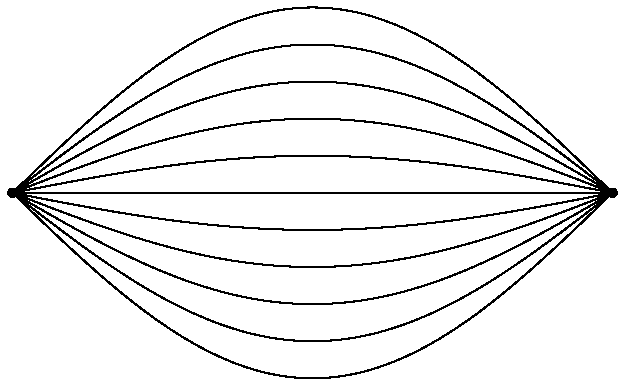
\includegraphics[width=3in]{../graphics/stand.pdf}
\]
Notice how the string is attached at the dots on the left and right?
Points like those are called \textit{nodes}\index{nodes}. While there
are many places that nodes can be, for us nodes will always be at the
endpoints of the string.

\begin{dfn} 
The \textbf{wavelength}\index{wavelength!standing wave} of a standing
wave is twice the length from node to node.
\end{dfn}

\begin{dfn} 
The \textbf{frequency}\index{frequency!standing wave} of a standing
wave is the number of complete vibrations (up and down) per unit time.
\end{dfn}

If we're talking about strings on instruments, then wavelength and
frequency are related by the following equation:
\begin{equation}\label{E:standing}
w_t \cdot f = c\qquad\text{where}\qquad
\begin{tabular}{l}
$w_t$ is the wavelength of the standing wave \\
$f$ is the frequency \\
\begin{minipage}{30ex}$c$ is a constant based on the mass and tension of the string\end{minipage}
\end{tabular}
\end{equation}

\begin{ques} 
If you pluck a string, what will the wavelength of the sound wave be?
Use equations (\ref{E:sin}) and (\ref{E:standing}) to express your
answer in terms of $w_t$, $f$, $c$ and $s$.
\end{ques}
\QM


\begin{ques} 
If you shorten a string's length by one-third, what will the
wavelength of the new sound wave be?  Use equations (\ref{E:sin}) and
(\ref{E:standing}) to express your answer in terms of $w_t$, $f$, $c$
and $s$.
\end{ques}
\QM

The upshot of the two questions above is that if you want to produce a
tone whose wavelength is a fraction of another tone's wavelength, then
your merely pluck a string whose length is the same fraction of the
string that produced the original tone. Let's get back to instrument building.

\begin{ques} 
When building a musical instrument, what tones do you want to be able
to play?
\end{ques}

I'll take this one! You want to be able to play tonic (open string),
the dominant, and the octave. How do we make this happen? Let's
imagine we are building a stringed instrument. Many stringed
instruments use \textit{frets}\index{frets} (little metal things that
help make new tones) to get the desired tones. To start, we'll want to
put a fret $2/3$ along the length of the string:
\[
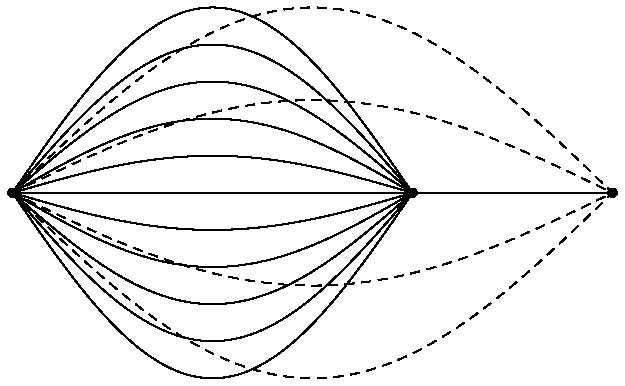
\includegraphics[width=3in]{../graphics/dom1.pdf}
\]
Additionally, we want to be able to play the dominant of this new tone
as well. To do this, we'll might place a new fret
\[
\frac{2}{3}\cdot \frac{2}{3} = \frac{4}{9}
\]
of the length of the string. 
\[
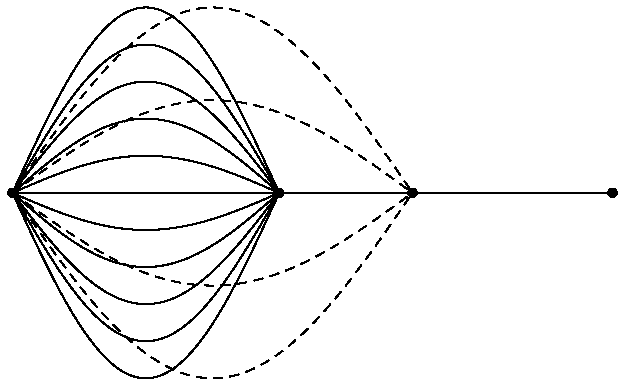
\includegraphics[width=3in]{../graphics/pdom2.pdf}
\]
Hmmmm there is a slight problem though. This new fret would create a
note \textit{higher} than the octave ($1/2$ the length of the
string). We want all of our frets to be placed between the original
tonic and octave. So let's move this fret over by lowering our new
tone by an octave. The new wavelength will be twice as long, so we'll
put a fret $8/9$ along the length of the string.
\[
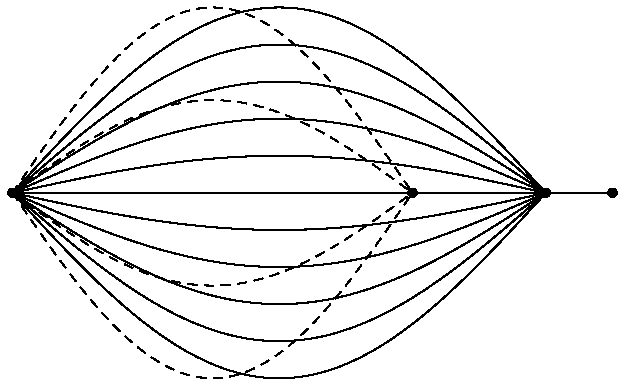
\includegraphics[width=3in]{../graphics/dom2.pdf}
\]
Now repeat this process, adding a new fret for the dominant of the
previously added tone, at each step ensuring that the fret be placed
between $1/2$ and complete string length. Do this $12$ times, let's
see what happens. Fill in the fractions in the boxes below---as a
gesture of friendship, I've given you the correct decimal approximation
for each fraction:
\[
\begin{array}{|r|c|c|c|c|c|c|}\hline
\text{fraction} &\rule[0mm]{0mm}{7mm}            &            &            &            &            &            \\ \hline
\bigstrut[t]\text{decimal}  & 0.666\dots & 0.888\dots & 0.592\dots & 0.790\dots & 0.526\dots & 0.702\dots \\ \hline
\end{array}
\]
\[
\begin{array}{|r|c|c|c|c|c|c|}\hline
\text{fraction}  &\rule[0mm]{0mm}{7mm}           &            &            &            &            &            \\ \hline
\bigstrut[t]\text{decimal}   & 0.936\dots & 0.624\dots & 0.832\dots & 0.554\dots & 0.739\dots & 0.493\dots \\ \hline
\end{array}
\]
From this we find we should place a twelfth fret $0.493\dots$ along
the length of the string. To the human ear, this tone will sound quite
close to the octave of our starting tone (though slightly
lower). Hence after twelve steps we \textit{appear} to be at the
octave. If we were to put frets on our instrument at all of these
divisions, we would have something like this:
\begin{equation}\label{E:fboard}
\begin{array}{c}
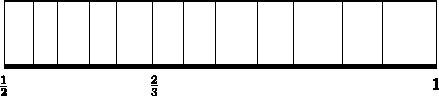
\includegraphics{../graphics/fboard1.pdf}
\end{array}
\end{equation}
Remember though, the twelfth fret is close to an octave, but not
perfect!  Mathematically we might say
\[
\frac{2^n}{3^m} \approx \frac{1}{2}
\]
for some integers $n$ and $m$. We note that in our case $m = 12$ and
$n$ is some other integer. Could we find integers $n$ and $m$ such that
\[
\frac{2^n}{3^m} =\frac{1}{2}?
\]
If so then we could write:
\[
2^{n+1} = 3^m \qquad\Leftrightarrow\qquad 2^{(n+1)/m} = 3
\]
\begin{ques}\index{Unique Factorization Theorem} 
What does the Unique Factorization Theorem for integers say about the
above expressions? How do we proceed from here?
\end{ques}
\QM 



\newpage

\subsection*{Problems for Section \thesection}\hrule\vspace{1ex}
\begin{enumerate}
\item Explain what the octave of a given tone is.
\item Explain what the dominant of given tone is.
%%
%% \item sketch the octave of a given tone!
%%
\item Order the following wavelengths by which tone they produce from
  lowest to highest.
\begin{align*}
&0.666\dots, 0.888\dots, 0.592\dots, 0.790\dots, 0.526\dots, 0.702\dots, \\
&0.936\dots, 0.624\dots, 0.832\dots, 0.554\dots, 0.739\dots, 0.493\dots
\end{align*}
Explain your reasoning.
\item Do the following tones sound ``right'' or ``wrong'' when played together?
\[
\begin{tabular}{ccc}
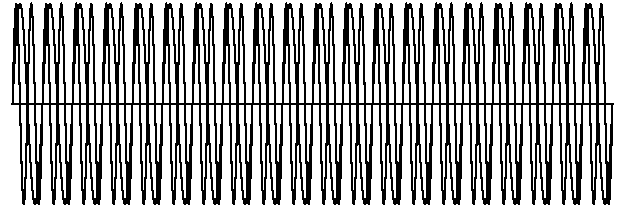
\includegraphics[width=2in]{../graphics/octaveComb.pdf}
 & \raisebox{4ex}{\huge$\Rightarrow$ }&
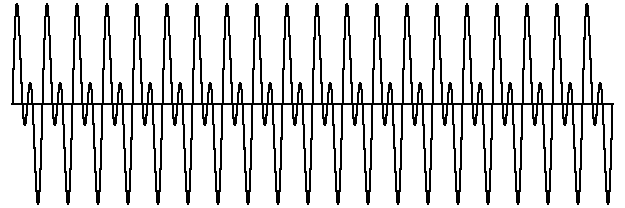
\includegraphics[width=2in]{../graphics/octaveSum.pdf}
\end{tabular}
\]
Explain your reasoning.
\item Do the following tones sound ``right'' or ``wrong'' when played together?
\[
\begin{tabular}{ccc}
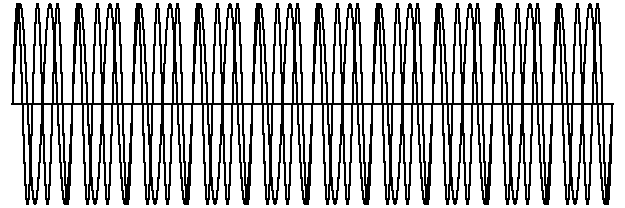
\includegraphics[width=2in]{../graphics/fifthComb.pdf}
 & \raisebox{4ex}{\huge$\Rightarrow$ }&
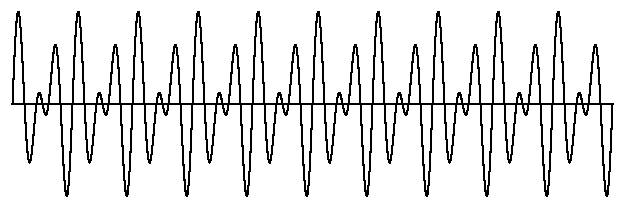
\includegraphics[width=2in]{../graphics/fifthSum.pdf}
\end{tabular}
\]
Explain your reasoning.
\item Do the following tones sound ``right'' or ``wrong'' when played together?
\[
\begin{tabular}{ccc}
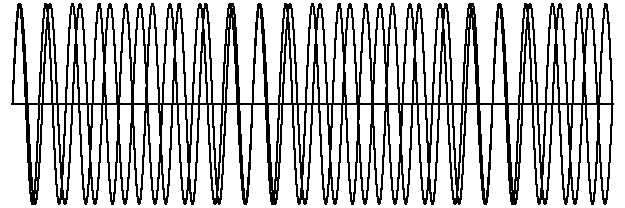
\includegraphics[width=2in]{../graphics/minorComb.pdf}
 & \raisebox{4ex}{\huge$\Rightarrow$ }&
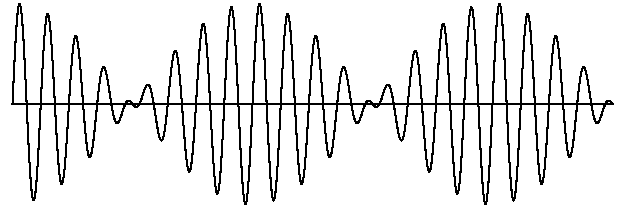
\includegraphics[width=2in]{../graphics/minorSum.pdf}
\end{tabular}
\]
Explain your reasoning.
\item Do the following tones sound ``right'' or ``wrong'' when played together?
\[
\begin{tabular}{ccc}
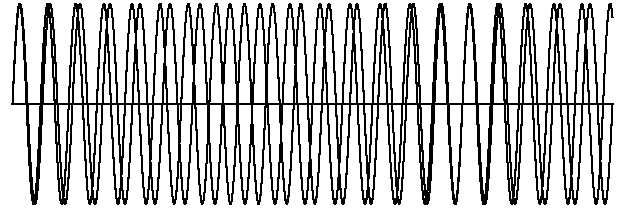
\includegraphics[width=2in]{../graphics/p2Comb.pdf}
 & \raisebox{4ex}{\huge$\Rightarrow$ }&
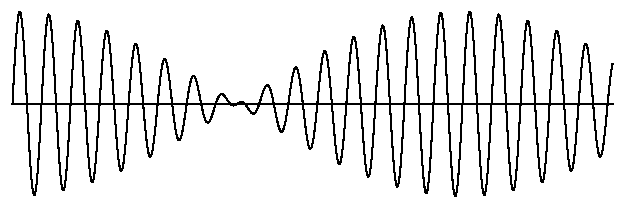
\includegraphics[width=2in]{../graphics/p2Sum.pdf}
\end{tabular}
\]
Explain your reasoning.
\item Do the following tones sound ``right'' or ``wrong'' when played together?
\[
\begin{tabular}{ccc}
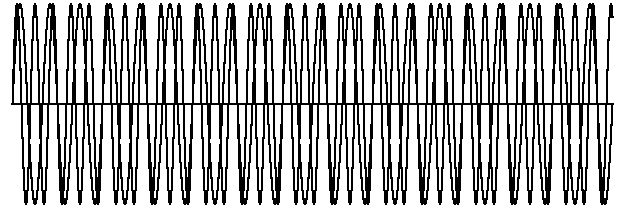
\includegraphics[width=2in]{../graphics/p1Comb.pdf}
 & \raisebox{4ex}{\huge$\Rightarrow$ }&
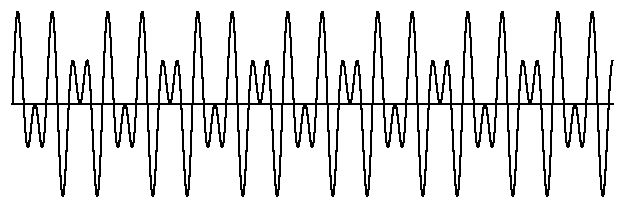
\includegraphics[width=2in]{../graphics/p1Sum.pdf}
\end{tabular}
\]
Explain your reasoning.
\item What is the wavelength of the dominant over the tone of
  wavelength $2/3$? Explain your reasoning.
\item What is the wavelength of the dominant over the tone of
  wavelength $3/4$? Explain your reasoning.
\item What is the wavelength of the dominant over the tone of
  wavelength $7/8$? Explain your reasoning.
\item What is the wavelength of the dominant over the tone of
  wavelength $6/13$? Explain your reasoning.
\item What is the wavelength of the dominant over the tone of
  wavelength $7/13$? Explain your reasoning.
\item What is the wavelength of the dominant over the tone of
  wavelength $2/3$ if we insist that the resulting wavelength is
  between $1/2$ and $1$? Explain your reasoning.
\item What is the wavelength of the dominant over the tone of
  wavelength $4/7$ if we insist that the resulting wavelength is
  between $1/2$ and $1$? Explain your reasoning.
\item What is the wavelength of the dominant over the tone of
  wavelength $5/8$ if we insist that the resulting wavelength is
  between $1/2$ and $1$? Explain your reasoning.
\item What is the wavelength of the dominant over the tone of
  wavelength $5/9$ if we insist that the resulting wavelength is
  between $1/2$ and $1$? Explain your reasoning.
\item What is the wavelength of the dominant over the tone of
  wavelength $6/11$ if we insist that the resulting wavelength is
  between $1/2$ and $1$? Explain your reasoning.
\item Give a precise derivation of how we obtained the fret positions
\begin{align*}
&0.666\dots, 0.888\dots, 0.592\dots, 0.790\dots, 0.526\dots, 0.702\dots, \\
&0.936\dots, 0.624\dots, 0.832\dots, 0.554\dots, 0.739\dots, 0.493\dots
\end{align*}
using the ideas of the tonic and dominant.

\end{enumerate}




\newpage


\section{Rational and Irrational Temperament}



In the last section, we were thinking about how to build a stringed
instrument with frets. With this in mind, we came up with the
following equation
\[
2^{\frac{n+1}{m}} = 3
\]
where $m$ is the number of divisions of the string that we would wish
to make. Armed with the Unique Factorization Theorem for
integers,\index{Unique Factorization Theorem} we could (and you will!)
explain that there is no rational solution of
\[
2^x = 3,
\]
meaning that  finding appropriate values of $n$ and $m$ is
actually impossible! It's a good thing that we are not the type of
people to be deterred by the impossible. In light of our discussion
above, we want to find a fraction:
\[
\frac{n+1}{m} \approx \log_2(3) = 1.58496250072115618145373894394\dots
\]

\begin{ques} 
How do we find good fractional approximations of irrational numbers?
\end{ques}

In two words: Continued fractions.\index{continued fraction} Set:
\[
x_1 = 1.58496250072115618145373894394\dots
\]
Write $x$ in terms of its whole-number part and its fractional part:
\[
x_1 = \mathbf{1} + (x_1-1)
\]
Now look at the reciprocal of $(x_1-1)$:
\begin{align*}
x_2 &=\frac{1}{x_1-1} = 1.70951129135145477697619026217\dots\\
x_2 &= \mathbf{1} + (x_2-1)
\end{align*}
Continue on:
\begin{align*}
x_3 &=\frac{1}{x_2-1} = 1.40942083965320900458240433081\dots\\
x_3 &= \mathbf{1} + (x_3-1)
\end{align*}
Again, again!
\begin{align*}
x_4 &=\frac{1}{x_3-1} = 2.44247459618085927548717403238\dots\\
x_4 &= \mathbf{2} + (x_4-2)
\end{align*}
One last time:
\begin{align*}
x_5 &=\frac{1}{x_4-2} = 2.26001675267082453593127612260\dots\\
x_5 &= \mathbf{2} + (x_5-2)
\end{align*}
Whew, now I'm tired, we could continue on but I think it is time to
stop. Let's see what our continued fraction looks like:
\[
\log_2(3) \approx 1 + \dfrac{1}{1+\dfrac{1}{1 + \dfrac{1}{2 + \dfrac{1}{2}}}}
\]
If we simplify this continued fraction into a regular old fraction we find:
\[
\log_2(3) \approx \frac{19}{12} = 1.58333333333\dots
\]
Check this out:
\[
2^{19/12} = 2.9966141537\dots
\]
This is really close to $3$, thus $2^{19/12}$ is a good approximation
of $\log_2(3)$. Write
\begin{align*}
3&\approx 2^{19/12} \\
\frac{2}{3} &\approx \frac{2}{2^{19/12}} \\
&\approx \frac{1}{2^{7/12}}
\end{align*}




With this in mind, we will adopt the convention that
the $n$th tone above the tonic will have a wavelength of exactly
$1/2^{n/12}$ of the tonic:
\[
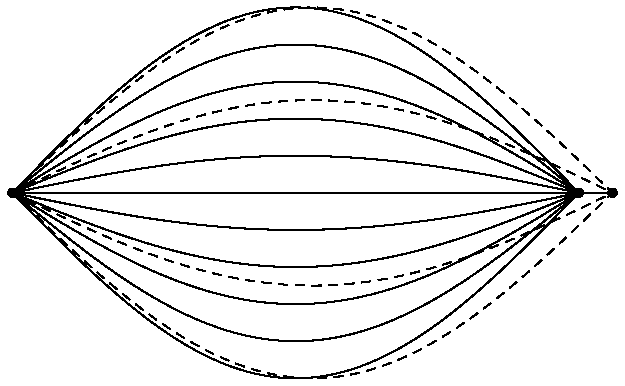
\includegraphics[width=3in]{../graphics/firstFret.pdf}
\]
In particular, since 
\[
\frac{1}{2^{1/12}} \cdot \frac{1}{2^{1/12}} = \frac{1}{2^{2/12}}
\]
if we work with wavelengths of $1/2^{n/12}$ of the tonic, we will
obtain a nice approximation of every tone we produced before. After
$7$ steps,
\[
\frac{1}{2^{7/12}} = 0.66741992\dots \approx \frac{2}{3}
\]
and additionally, 
\[
\frac{1}{2^{12/12}} = \frac{1}{2},
\]
so after twelve steps we are exactly at the octave! If we put a frets
at the points $\frac{1}{2^{n/12}}$ letting $n$ run from $0$ to $12$, we'll obtain a picture like:
\[
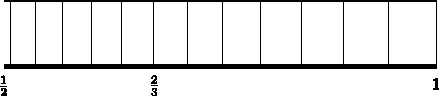
\includegraphics{../graphics/eqFret.pdf}
\]
Let's compare this to our fret positions in diagram~(\ref{E:fboard}):
\[
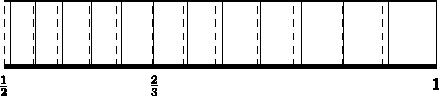
\includegraphics{../graphics/bFret.pdf}
\]
\begin{ques} Will this really work?
\end{ques}
\QM

\subsection{Equal Temperament}

Spacing the division of the tones by making use of wavelengths that
are $\frac{1}{2^{1/12}}$ of the tonic is called \textbf{equal
  temperament}\index{equal temperament}. This is how modern guitars
and pianos are tuned. People have also identified other ratios of the
wavelength of the tonic that they thought sounded ``right.''
Essentially, they have taken the idea that we should have as few
``beats'' as possible to the extreme. When they do this, and attempt
to have $12$ tones, they arrive at what is called \textbf{just
  intonation}\index{just intonation}. When \textit{a
  cappella}\index{\textit{a cappella}@acappella} groups sing and form
chords, they usually sing using just intonation---the human brain
seems to be somehow drawn to these sounds. Here are the ratios of the
wavelength of the tonic used in just intonation:
\begin{align*}
&1/2,\quad 8/15,\quad 5/9,\quad 3/5,\quad 5/8,\quad 2/3,\\
&32/45,\quad 3/4,\quad 4/5,\quad 5/6,\quad 8/9,\quad 24/25
\end{align*}
Let's compare these to the ratios used in equal temperament:
\[
\begin{tabular}{rr@{\,}c@{\,}lr@{\,}c@{\,}l}
Tone & \multicolumn{3}{c}{Equal Temperament}   & \multicolumn{3}{c}{Just Intonation}   \\ \hline
\bigstrut[t] $12$ & $1/2^{12/12}$ & $=$ & $0.5$         & $1/2$   & $=$& $0.5$      \\
$11$ & $1/2^{11/12}$ & $=$ & $0.529\dots$  & $8/15$  & $=$& $0.533\dots$ \\
$10$ & $1/2^{10/12}$ & $=$ & $0.561\dots$  & $5/9$   & $=$& $0.555\dots$    \\
$9$  & $1/2^{9/12}$  & $=$ & $0.594\dots$  & $3/5$   & $=$& $0.6$ \\
$8$  & $1/2^{8/12}$  & $=$ & $0.629\dots$  & $5/8$   & $=$& $0.625$ \\
$7$  & $1/2^{7/12}$  & $=$ & $0.667\dots$  & $2/3$   & $=$& $0.666\dots$ \\
$6$  & $1/2^{6/12}$  & $=$ & $0.707\dots$  & $32/45$ & $=$& $0.711\dots$ \\
$5$  & $1/2^{5/12}$  & $=$ & $0.749\dots$  & $3/4$   & $=$& $0.75$ \\
$4$  & $1/2^{4/12}$  & $=$ & $0.793\dots$  & $4/5$   & $=$& $0.8$ \\
$3$  & $1/2^{3/12}$  & $=$ & $0.840\dots$  & $5/6$   & $=$& $0.833\dots$ \\
$2$  & $1/2^{2/12}$  & $=$ & $0.890\dots$  & $8/9$   & $=$& $0.888\dots$ \\
$1$  & $1/2^{1/12}$  & $=$ & $0.943\dots$  & $24/25$ & $=$& $0.96\dots$ \\ \hline
\end{tabular}
\]
The real issue with just intonation comes with we try to raise every
note up by a given number of steps. Suppose a singer has trouble
singing in the range of some song, yet has no problems if we raise
every note of the song up by $1$ half step. If our instrument is in
equal temperament, then this shift of tones will have no adverse
effects. However, if our instrument is in just intonation, then check
out what happens:
\begin{itemize}
\item Let $24/25$ of a wavelength be the new tonic---this is 1 half
  step.
\item Now $7$ steps up will be $5/8$ of a wavelength.
\end{itemize}
Checking out the new ratio we find:
\[
\frac{5/8}{24/25} = 0.651042 
\]  
This is over a $2 \%$ difference from $2/3$ of the tonic. Believe it
or not, this will be noticeably ``wrong'' to the human ear. With
equal temperament, the tone will still be spot-on.

These issues with musical instruments arise due to intrinsic
differences between rational and irrational numbers. The tones that
sound best to our ears are all defined by ratios of the wavelength of
the tonic. However, moving up by these ratios is done via
multiplication, and hence logarithms enter the scene. The Unique
Factorization Theorem for integers\index{Unique Factorization Theorem}
tells us that the ratios that we are most interested in cannot be
obtained simply from the other ratios we are interested in. From all
this arises a fascinating problem that everyone experiences without
even realizing it!


\newpage

\subsection*{Problems for Section \thesection}\hrule\vspace{1ex}
\begin{enumerate}
\item Explain why $\log_2(3)$ is an irrational number.
\item Explain why $\log_3(5)$ is an irrational number.
\item Explain why $\log_3(6)$ is an irrational number.
\item Explain why $\log_4(6)$ is an irrational number.
\item Explain why $\log_9(10)$ is an irrational number.
\item Find the simple continued fraction expansion of $5/3$. Explain
  your reasoning.
\item Find the simple continued fraction expansion of $15/11$. Explain
  your reasoning.
\item Find the simple continued fraction expansion of $22/17$. Explain
  your reasoning.
\item Using a calculator, find the first five terms in the simple
  continued fraction expansion of $e$. What number do you get by only
  considering the first term? The first two terms? The first three
  terms? The first four? The first five?  Explain your reasoning.
\item Using a calculator, find the first five terms in the simple
  continued fraction expansion of $\pi$. What number do you get by
  only considering the first term? The first two terms? The first
  three terms? The first four? The first five?  Explain your
  reasoning.
\item Suppose you are building a stringed instrument. If the first
  octave of $12$ tones has a length of $16$ inches, how long is the
  next octave? What about the next octave? Explain your reasoning.
\item A singer and a piano are playing a chord involving the sixth
  tone. If the singer is singing in just intonation, and the piano is
  in equal temperament, does the singer believe that the piano is
  playing too high or too low? Explain your reasoning.
\item A singer and a piano are playing a chord involving the seventh
  tone. If the singer is singing in just intonation, and the piano is
  in equal temperament, does the singer believe that the piano is
  playing too high or too low? Explain your reasoning.
\item A singer and a piano are playing a chord involving the fourth
  tone. If the singer is singing in just intonation, and the piano is
  in equal temperament, does the singer believe that the piano is
  playing too high or too low? Explain your reasoning.
\item A singer and a piano are playing a chord involving the twelfth
  tone. If the singer is singing in just intonation, and the piano is
  in equal temperament, does the singer believe that the piano is
  playing too high or too low? Explain your reasoning.
\item Some other cultures place $5$ tones between octaves. Can you
  explain this if you know that they are trying to approximate
  $\log_2(3)$?
\item Light also has wave-like properties. The wavelengths of the
  visible spectrum goes from around $380$ nm to $750$ nm. Sometimes
  colors are depicted as being in a line, other times they are
  depicted as being in a wheel. Can you use our discussion on music,
  thinking about tonics and octaves to give a plausible resolution to
  this paradox?

%\item The tone whose wavelength is $3/4$ that of the tonic is called
%  the \textbf{sub-dominant}.\index{sub-dominant} If we try to base a
%  tuning system on this tone, we end up trying to approximate
%  $\log_3{4}$. Can you explain why when people did this, they arrived
%  at a $19$ tone system?


%4/3 sub-dominant
%5:4 mediant
\end{enumerate}

